\begin{tikzpicture}
  [elm/.style={draw, align=center, text width=.6cm}]
  \node[elm, fill=LightCyan] (h1) {0};
  \node[elm, fill=LightCyan, right of=h1] (h2) {1};
  \node[elm, fill=MistyRose, right of=h2] (h3) {2};
  \node[elm, fill=MistyRose, right of=h3] (h4) {3};    
  \foreach \i in {5,...,40}{
    \pgfmathtruncatemacro{\y}{\i-1};
    \node[elm, right of=h\y] (h\i) {\y}; 
  }
\end{tikzpicture}
